\documentclass[10pt, aspectratio=169]{beamer}

%\usepackage[top = 1 in, bottom = 1 in, left = 1 in, right = 1 in]{geometry}

\usepackage{amsmath}
\allowdisplaybreaks[1]
\usepackage{amssymb, amsfonts}
\usepackage{enumerate}
\usepackage{multirow}
\usepackage{hhline}
\usepackage{array}
\usepackage{longtable}
\usepackage{mathrsfs}
\usepackage{graphicx}
\usepackage{tabularray}
\usepackage{undertilde}
\usepackage{dingbat}
\usepackage{fontawesome5}
\usepackage{tasks}
\usepackage{bbding}
\usepackage{hyperref}
\usepackage[linesnumbered,ruled,vlined]{algorithm2e}
\usepackage{twemojis}
% how to use bull's eye ----- \scalebox{2.0}{\twemoji{bullseye}}
\usepackage{customdice}
% how to put dice face ------ \dice{2}
\usepackage{pgfplots}
\pgfplotsset{compat=1.17}

\usepackage{fontspec}
\setmainfont{Century Schoolbook}
\renewcommand{\familydefault}{\rmdefault}

\usepackage{unicode-math}
%\setmathfont{Latin Modern Math}
\setmathfont{XITS Math}

\usepackage{tikz}
\usetikzlibrary{arrows.meta}
\usetikzlibrary{patterns}

\usetheme{Warsaw}
\setbeamertemplate{headline}{}
\setbeamertemplate{footline}[page number in head/foot]{}
\usecolortheme{default}

\setbeamercolor{block title}{fg=blue!80!black, bg=blue!20}
\setbeamercolor{block body}{fg=black, bg=blue!5}

\usetikzlibrary{overlay-beamer-styles}
\usetikzlibrary{positioning}
\usetikzlibrary{calc}

\title{Gradient Descent and Siblings}
\author[\href{mailto:ami.ananda@bhu.ac.in}{\faEnvelope \, ami.ananda@bhu.ac.in}]{Ananda Biswas \\[0.5em] \href{mailto:ami.ananda@bhu.ac.in}{\faEnvelope \, ami.ananda@bhu.ac.in}}
\date{}


\begin{document}


\begin{frame}
	\titlepage
\end{frame}

\begin{frame}
	\begin{block}{Acknowledgements}
		\begin{itemize}
		\item CS7015 Lectures\footnote{\href{https://www.youtube.com/playlist?list=PLyqSpQzTE6M9gCgajvQbc68Hk_JKGBAYT}{YouTube}} of Professor Mitesh Khapra \\[0.75em]
		\item Videos\footnote{\href{https://www.youtube.com/playlist?list=PLEAYkSg4uSQ2WG11drrwV6Igj360RaxK9}{YouTube}} of Ryan Harris on Backpropagation
		\end{itemize}			
	\end{block}
\end{frame}


\begin{frame}{Target : Learning Parameters}
\centering
\begin{tikzpicture}[
    node distance=4cm,
    box/.style={draw, minimum width=2cm, minimum height=1cm, font=\ttfamily}
]
    % Nodes
    \only<1->{\node[box] (head) {Supervised Learning};}
    \only<2->{\node[box, right of=head] (n1) {Loss $\mathscr{L}(\symbf{\theta})$};}
    \only<3->{\node[box, right of=n1] (n2) {optimal $\symbf{\theta}$};}

    % Arrows
    \only<2->{\draw[-{Latex}] (head) -- (n1);}
    \only<3->{\draw[-{Latex}] (n1) -- (n2);}
\end{tikzpicture}
\end{frame}

\begin{frame}{Set-up}
\begin{columns}
	\begin{column}{0.5\textwidth}
	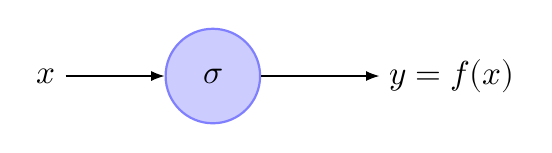
\begin{tikzpicture}[
    node distance=1.5cm and 1.5cm,
    every node/.style={font=\large},
    neuron/.style={circle, draw=blue!50, fill=blue!20, thick, minimum size=1.2cm}]
    
% Nodes
\node (x) {$x$};
\node[neuron, right=of $(x)$] (sigma) {$\sigma$};
\node[right=of sigma] (y) {$y = f(x)$};

% Arrows
\draw[-{Latex}] (x) -- (sigma);
\draw[-{Latex}] (sigma) -- (y);
\end{tikzpicture}

\[
f(x) = \dfrac{1}{1 + e^{-(wx + b)}}
\]
	\end{column}
	
	\begin{column}{0.5\textwidth}
	\begin{block}{Input for Training}
	$(x_i, y_i)_{i = 1}^{n}$ \rightarrow  $n$ pairs of $(x, y)$
	\end{block}
	
	\begin{block}{Training Objective}
	Find $w$ and $b$ that minimizes \\[0.75em]
	
	$$\mathscr{L}(w, b) = \sum \limits_{i = 1}^{n} \left(y_i - f(x_i)^2\right)$$
	\end{block}

	\end{column}
\end{columns}
\end{frame}


\begin{frame}{Set-up}

\begin{columns}
\begin{column}{0.5\textwidth}
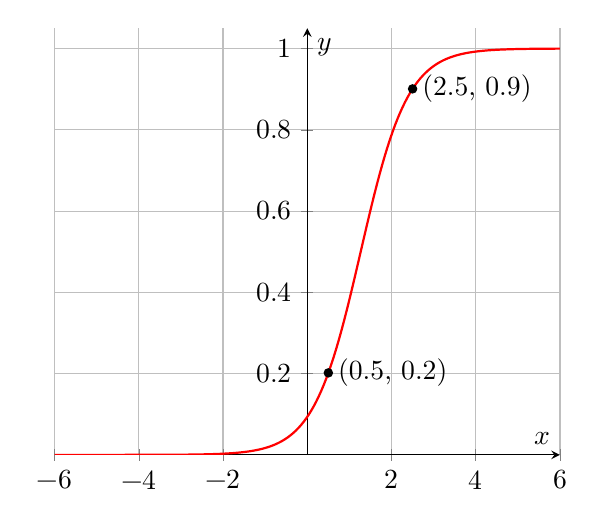
\begin{tikzpicture}
\begin{axis}[
    axis lines=middle,
    xlabel={$x$},
    ylabel={$y$},
    xmin=-6, xmax=6,
    ymin=0, ymax=1.05,
    domain=-6:6,
    samples=200,
    grid=both,
    width=8cm,
    height=7cm
]

% Logistic function plot
\only<2->{\addplot[red, thick] {1/(1+exp(-(1.79*x - 2.27))};}

% First point
\addplot[
    mark=*,
    only marks,
    mark size=1.5pt
] coordinates {(0.5, {1/(1+exp(-(1.79*0.5 - 2.27))})};
\node[anchor=west] at (axis cs:0.5, {1/(1+exp(-(1.79*0.5 - 2.27))}) {(0.5, 0.2)};

% Second point
\addplot[
    mark=*,
    only marks,
    mark size=1.5pt
] coordinates {(2.5, {1/(1+exp(-(1.79*2.5 - 2.27))})};
\node[anchor=west] at (axis cs:2.5, {1/(1+exp(-(1.79*2.5 - 2.27))}) {(2.5, 0.9)};

\end{axis}
\end{tikzpicture}
\end{column}

\begin{column}{0.5\textwidth}
\begin{block}{What is training ?}
	At the end of the process we wish to get $w^{*}$ and $b^{*}$ so that $f(0.5) \rightarrow 0.2$ and $f(2.5) \rightarrow 0.9$. \\[0.75em]
	
	\only<2->{In other words, we hope to find a sigmoid function that satisfies $(0.5, 0.2)$ and $(2.5, 0.9)$.}
	\end{block}
\end{column}
\end{columns}

\end{frame}


\begin{frame}{Approach 1 : Guess Work}

\begin{columns}
\begin{column}{0.5\textwidth}
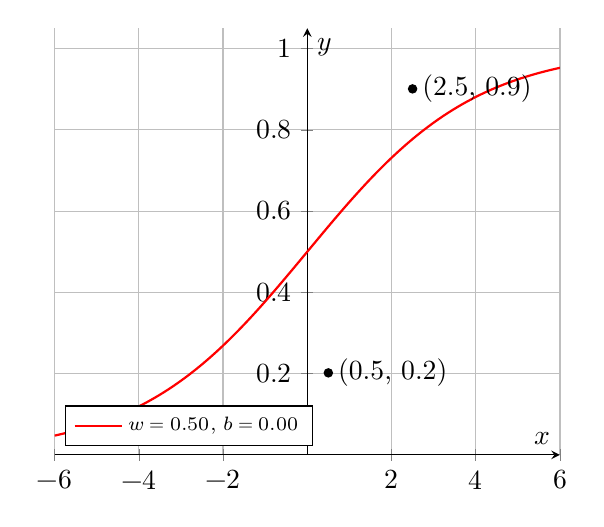
\begin{tikzpicture}
\begin{axis}[
    axis lines=middle,
    xlabel={$x$},
    ylabel={$y$},
    xmin=-6, xmax=6,
    ymin=0, ymax=1.05,
    domain=-6:6,
    samples=200,
    grid=both,
    width=8cm,
    height=7cm,
    legend style={
    at={(0.02,0.02)},
    anchor=south west,
    font=\scriptsize
}
]

% Logistic function plot
\only<2->{\addplot[red, thick] {1/(1+exp(-(0.5*x - 0.0))};
\addlegendentry{$w=0.50,\,b=0.00$}}

% First point
\addplot[
    mark=*,
    only marks,
    mark size=1.5pt
] coordinates {(0.5, {1/(1+exp(-(1.79*0.5 - 2.27))})};
\node[anchor=west] at (axis cs:0.5, {1/(1+exp(-(1.79*0.5 - 2.27))}) {(0.5, 0.2)};

% Second point
\addplot[
    mark=*,
    only marks,
    mark size=1.5pt
] coordinates {(2.5, {1/(1+exp(-(1.79*2.5 - 2.27))})};
\node[anchor=west] at (axis cs:2.5, {1/(1+exp(-(1.79*2.5 - 2.27))}) {(2.5, 0.9)};

\end{axis}
\end{tikzpicture}
\end{column}

\begin{column}{0.5\textwidth}
Let us try a random guess.. \\
\only<2->{say, $w = 0.5, b = 0$ \\}
\only<3->{Clearly not good, but how bad is it ? \\[1em]}
\only<4->{$\mathscr{L}(w, b) = \sum \limits_{i = 1}^{n} \left(y_i - f(x_i)^2\right)$ will tell us.}

\end{column}
\end{columns}
\end{frame}

\begin{frame}

\begin{columns}
\begin{column}{0.5\textwidth}
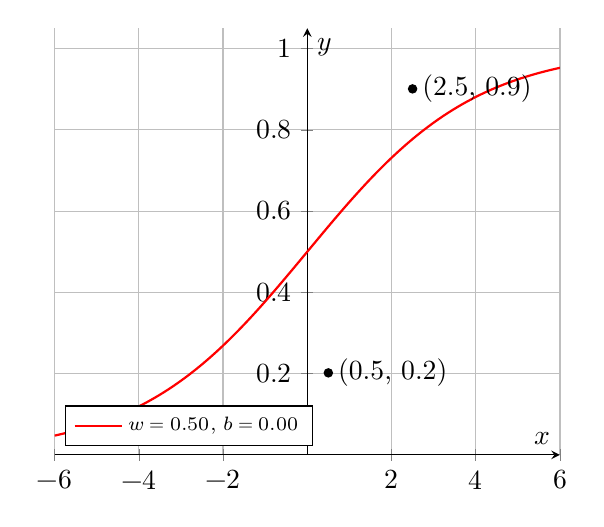
\begin{tikzpicture}
\begin{axis}[
    axis lines=middle,
    xlabel={$x$},
    ylabel={$y$},
    xmin=-6, xmax=6,
    ymin=0, ymax=1.05,
    domain=-6:6,
    samples=200,
    grid=both,
    width=8cm,
    height=7cm,
    legend style={
    at={(0.02,0.02)},
    anchor=south west,
    font=\scriptsize
}
]

% Logistic function plot
\addplot[red, thick] {1/(1+exp(-(0.5*x - 0.0))};
\addlegendentry{$w=0.50,\,b=0.00$}

% First point
\addplot[
    mark=*,
    only marks,
    mark size=1.5pt
] coordinates {(0.5, {1/(1+exp(-(1.79*0.5 - 2.27))})};
\node[anchor=west] at (axis cs:0.5, {1/(1+exp(-(1.79*0.5 - 2.27))}) {(0.5, 0.2)};

% Second point
\addplot[
    mark=*,
    only marks,
    mark size=1.5pt
] coordinates {(2.5, {1/(1+exp(-(1.79*2.5 - 2.27))})};
\node[anchor=west] at (axis cs:2.5, {1/(1+exp(-(1.79*2.5 - 2.27))}) {(2.5, 0.9)};

\end{axis}
\end{tikzpicture}
\end{column}

\begin{column}{0.5\textwidth}
\begin{align*}
\mathscr{L}(w, b) &= \sum \limits_{i = 1}^{n} \left(y_i - f(x_i)^2\right) \\[0.5em]
&= \dfrac{1}{2} \left[ \left( y_1 - f(x_1) \right)^2 + \left( y_2 - f(x_2) \right)^2 \right] \\[0.5em]
&= \dfrac{1}{2} \left[ \left( 0.2 - f(0.5) \right)^2 + \left( 0.9 - f(0.2) \right)^2 \right] \\[0.5em]
&= 0.073
\end{align*}

We want $\mathscr{L}(w, b) = \sum \limits_{i = 1}^{n} \left(y_i - f(x_i)^2\right)$ to as close to $0$ as possible.
\end{column}
\end{columns}
\end{frame}


\begin{frame}{Approach 1 : Guess Work}
\begin{columns}
\begin{column}{0.7\textwidth}
\begin{tikzpicture}
\begin{axis}[
    axis lines=middle,
    xlabel={$x$},
    ylabel={$y$},
    xmin=-6, xmax=6,
    ymin=0, ymax=1.05,
    domain=-6:6,
    samples=200,
    grid=both,
    width=10cm,
    height=7cm,
    legend style={
    at={(0.02,0.02)},
    anchor=south west,
    font=\scriptsize
}
]

% Functions
\only<1->{\addplot[red, thick] {1/(1+exp(-(0.50*x + 0.00)))};
\addlegendentry{$w=0.50,\,b=0.00$}}

\only<2->{\addplot[blue, thick] {1/(1+exp(-(-0.10*x + 0.00)))};
\addlegendentry{$w=-0.10,\,b=0.00$}}

\only<3->{\addplot[green, thick] {1/(1+exp(-(0.94*x - 0.95)))};
\addlegendentry{$w=0.94,\,b=-0.95$}}

\only<4->{\addplot[purple, thick] {1/(1+exp(-(1.43*x - 1.74)))};
\addlegendentry{$w=1.43,\,b=-1.74$}}

\only<5->{\addplot[cyan, thick] {1/(1+exp(-(1.65*x - 2.08)))};
\addlegendentry{$w=1.65,\,b=-2.08$}}

\only<6->{\addplot[orange, thick] {1/(1+exp(-(1.78*x - 2.27)))};
\addlegendentry{$w=1.78,\,b=-2.27$}}

% First point
\addplot[
    mark=*,
    only marks,
    mark size=1.5pt
] coordinates {(0.5, {1/(1+exp(-(1.79*0.5 - 2.27))})};
\node[anchor=west] at (axis cs:0.5, {1/(1+exp(-(1.79*0.5 - 2.27))}) {(0.5, 0.2)};

% Second point
\addplot[
    mark=*,
    only marks,
    mark size=1.5pt
] coordinates {(2.5, {1/(1+exp(-(1.79*2.5 - 2.27))})};
\node[anchor=west] at (axis cs:2.5, {1/(1+exp(-(1.79*2.5 - 2.27))}) {(2.5, 0.9)};

\end{axis}
\end{tikzpicture}
\end{column}

\begin{column}{0.3\textwidth}
\only<1->{We try with some other values of $w$ and $b$.}

\begin{table}[!htbp]
\def\arraystretch{1.5}

\begin{center}
\begin{tabular}{ccc}

\hline
$w$ & $b$ & $\mathscr{L}(w, b)$ \\

\hline
\hline
$0.50$ & $0.00$ & $0.0730$ \\
\only<2->{$-0.10$ & $0.00$ & $0.1481$} \\
\only<3->{$0.94$ & $-0.94$ & $0.0214$} \\
\only<4->{$1.42$ & $-1.73$ & $0.0028$} \\
\only<5->{$1.65$ & $-2.08$ & $0.0003$} \\
\only<6->{$1.78$ & $-2.27$ & $0.0000$} \\
\hline
\end{tabular}
\end{center}
\end{table}

\onslide<7->{Job done ! But}
\begin{itemize}
\item<8-> Infeasible
\item<9-> Does not gurantee correct solution
\end{itemize}
\end{column}
\end{columns}
\end{frame}


\begin{frame}{Approach 2 : Brute$-$force Search}
\centering
\begin{tikzpicture}[
    node distance=7cm,
    box/.style={draw, minimum width=2cm, minimum height=1cm, font=\ttfamily}
]
    % Nodes
    \only<1->{\node[box] (head) {Compute $\mathscr{L}(w, b)$ for all possible $w$ and $b$};}
    \only<2->{\node[box, right of=head] (n1) {Choose the best $w$ and $b$};}

    % Arrows
    \only<2->{\draw[-{Latex}] (head) -- (n1);}
\end{tikzpicture}

\vspace{2cm}

\onslide<3->{$\bullet$ Computationally infeasible}
\end{frame}

\begin{frame}{Revisit to Approach 1}
\begin{columns}
\begin{column}{0.5\textwidth}
\begin{tikzpicture}
\begin{axis}[
    axis lines=middle,
    xlabel={$x$},
    ylabel={$y$},
    xmin=-6, xmax=6,
    ymin=0, ymax=1.05,
    domain=-6:6,
    samples=200,
    grid=both,
    width=8cm,
    height=7cm,
    legend style={
    at={(0.001,0.02)},
    anchor=south west,
    font=\scriptsize
}
]

% Functions
\only<1->{\addplot[red, thick] {1/(1+exp(-(0.50*x + 0.00)))};
\addlegendentry{$w=0.50,\,b=0.00$}}

\only<2->{\addplot[blue, thick] {1/(1+exp(-(-0.10*x + 0.00)))};
\addlegendentry{$w=-0.10,\,b=0.00$}}

\only<3->{\addplot[green, thick] {1/(1+exp(-(0.94*x - 0.95)))};
\addlegendentry{$w=0.94,\,b=-0.95$}}

\only<4->{\addplot[purple, thick] {1/(1+exp(-(1.43*x - 1.74)))};
\addlegendentry{$w=1.43,\,b=-1.74$}}

\only<5->{\addplot[cyan, thick] {1/(1+exp(-(1.65*x - 2.08)))};
\addlegendentry{$w=1.65,\,b=-2.08$}}

\only<6->{\addplot[orange, thick] {1/(1+exp(-(1.78*x - 2.27)))};
\addlegendentry{$w=1.78,\,b=-2.27$}}

% First point
\addplot[
    mark=*,
    only marks,
    mark size=1.5pt
] coordinates {(0.5, {1/(1+exp(-(1.79*0.5 - 2.27))})};
\node[anchor=west] at (axis cs:0.5, {1/(1+exp(-(1.79*0.5 - 2.27))}) {(0.5, 0.2)};

% Second point
\addplot[
    mark=*,
    only marks,
    mark size=1.5pt
] coordinates {(2.5, {1/(1+exp(-(1.79*2.5 - 2.27))})};
\node[anchor=west] at (axis cs:2.5, {1/(1+exp(-(1.79*2.5 - 2.27))}) {(2.5, 0.9)};

\end{axis}
\end{tikzpicture}
\end{column}

\begin{column}{0.5\textwidth}
What we were actually doing !

\only<1>{
\begin{figure}
\centering
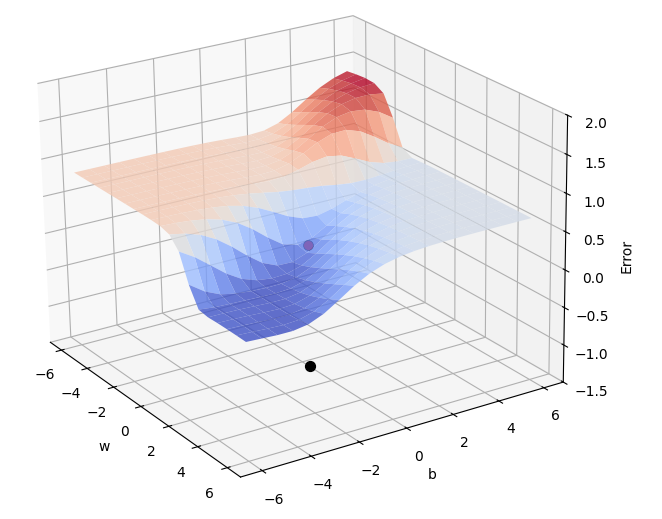
\includegraphics[scale=0.45]{Figure_1}
\end{figure}
}

\only<2>{
\begin{figure}
\centering
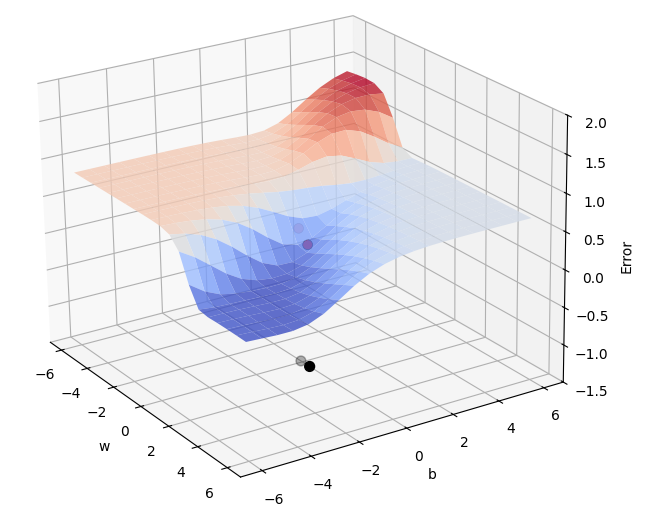
\includegraphics[scale=0.45]{Figure_2}
\end{figure}
}

\only<3>{
\begin{figure}
\centering
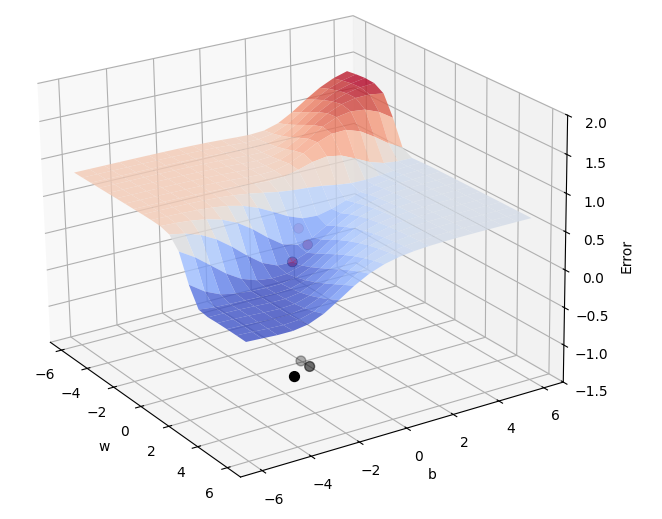
\includegraphics[scale=0.45]{Figure_3}
\end{figure}
}

\only<4>{
\begin{figure}
\centering
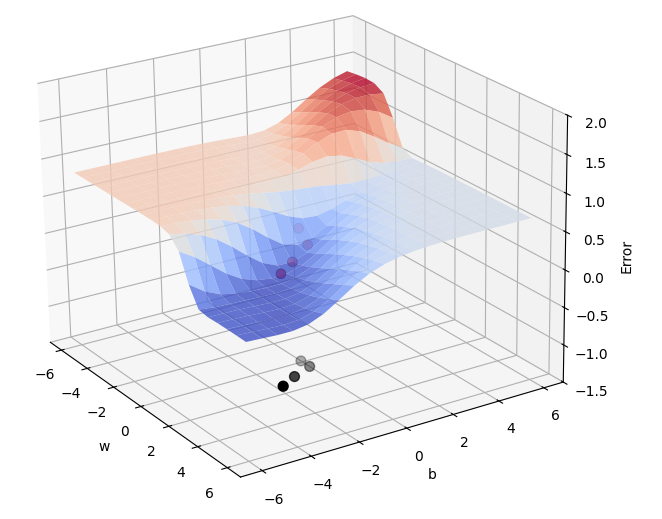
\includegraphics[scale=0.45]{Figure_4}
\end{figure}
}

\only<5>{
\begin{figure}
\centering
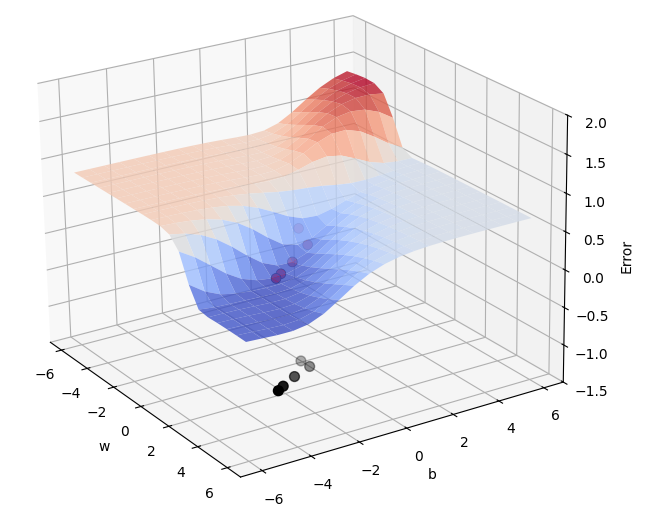
\includegraphics[scale=0.45]{Figure_5}
\end{figure}
}

\only<6>{
\begin{figure}
\centering
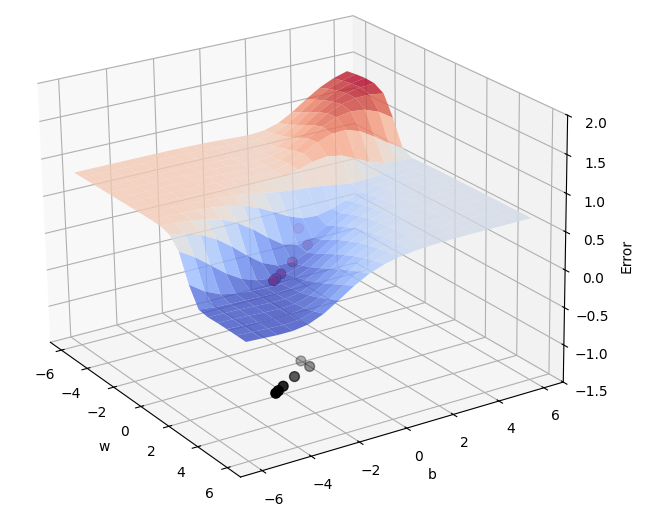
\includegraphics[scale=0.45]{Figure_6}
\end{figure}
}

\end{column}
\end{columns}
\end{frame}


\begin{frame}

\only<1->{
\begin{block}{So far ...}
We were traversing the error surface by fiddling with $w$ and $b$ with mere intuition and guess work.
\end{block}
}

\only<2->{
\begin{block}{Up next ...}
Looking for a more efficient and principled way of doing this.
\end{block}
}

\end{frame}

\begin{frame}
\begin{block}{\scalebox{2.0}{\twemoji{bullseye}} \hspace{0.1cm} Goal ahead}
To find a better way of traversing the error surface so that we can reach the minimum value quickly without resorting to guess work or brute force search which is any how infeasible.
\end{block}
\end{frame}


\begin{frame}{Approach 3 : A Principled Way}

\begin{columns}

\begin{column}{0.5\textwidth}
\begin{tikzpicture}[>=stealth, thick]

% Coordinates
\coordinate (O) at (0,0);      % origin
\coordinate (A) at (1.5,3);      % theta
\coordinate (B) at (4,0);      % delta theta
\coordinate (C) at ($(A)+(B)$);% theta + delta theta
\coordinate (D) at ($(O)!0.4!(B)$); % eta*delta theta
\coordinate (E) at ($(A)+(D)$);     % theta + eta*delta theta

% Black parallelogram edges
\only<1->{\draw[->] (O) -- (A) node[midway,left]{$\symbf{\theta}$};}
\only<2->{\draw[->] (O) -- (B) node[midway,below]{$\Delta \symbf{\theta}$};}
\only<3->{\draw[dashed] (A) -- (C);}
\only<3->{\draw[dashed] (B) -- (C);}
\only<3->{\draw[->] (O) -- (C) node[midway,sloped,above]{$\symbf{\theta}_{\text{new}}$};}


% Red eta * delta theta
\only<4->{\draw[red,->] (O) -- (D) node[midway,below]{$\eta \cdot \Delta \symbf{\theta}$};}

% Red theta_new
\only<5->{
\draw[red,->] (O) -- (E) node[midway,sloped,above]{$\symbf{\theta}_{\text{new}}$};
\draw[red,dashed] (A) -- (E);
\draw[red,dashed] (D) -- (E);
}
\end{tikzpicture}
\end{column}

\begin{column}{0.5\textwidth}
\begin{itemize}
\item<1-> Suppose we have a randomly initialized vector of parameters $\symbf{\theta} = \left[ w, b \right]$.

\item<2-> Let $\Delta\symbf{\theta} = \left[ \Delta w, \Delta b \right]$ denote change in the values of $w$ and $b$ respectively. 

\item<3-> So we move in the direction of $\Delta\symbf{\theta}$.

\item<4-> Let us be a bit conservative: we move only by a small amount $\eta > 0$.

\item<5-> $\symbf{\theta}_{new} = \symbf{\theta} + \eta \cdot \Delta\symbf{\theta}$

\item<6-> Now the question is what is the right $\Delta\symbf{\theta}$ to use. 

\item<7-> The answer comes from Taylor Series.
\end{itemize}
\end{column}
\end{columns}

\end{frame}

\begin{frame}
\only<1->{
\begin{block}{Taylor Series}
For a function $\mathcal{F}({x})$ expanded around ${a} \in \mathbb{R}$, we have,
$$\mathcal{F}({x}) = \mathcal{F}({a}) + ({x} - {a}) \mathcal{F'}({a}) + \dfrac{1}{2!} ({x} - {a})^2 {F''}({a}) + \cdots$$
\end{block}
}

\only<2->{
\begin{block}{Multivariate Taylor Series}
For a function $\mathcal{F}(\mathbf{x})$ expanded around $\mathbf{a} \in \mathbb{R}^n$, we have,
$$\mathcal{F}(\mathbf{x}) = \mathcal{F}(\mathbf{a}) + (\mathbf{x} - \mathbf{a})' \nabla \mathcal{F}(\mathbf{a}) + \dfrac{1}{2!} (\mathbf{x} - \mathbf{a})' \nabla^2 \mathcal{F}(\mathbf{a}) (\mathbf{x} - \mathbf{a}) + \cdots$$
\end{block}
}
\end{frame}


\begin{frame}
$$\mathcal{F}(\mathbf{x}) = \mathcal{F}(\mathbf{a}) + (\mathbf{x} - \mathbf{a})' \nabla \mathcal{F}(\mathbf{a}) + \dfrac{1}{2!} (\mathbf{x} - \mathbf{a})' \nabla^2 \mathcal{F}(\mathbf{a}) (\mathbf{x} - \mathbf{a}) + \cdots$$

\onslide<1->{For ease of notation, take $\Delta \symbf{\theta} = \symbf{u}$.} \\[0.8em]

\onslide<2->{With $\mathcal{F} = \mathscr{L}$ (our Loss Function),} \\
\onslide<2->{\hspace{0.8cm} $\mathbf{x} = \symbf{\theta} + \eta \symbf{u}$,} \\
\onslide<2->{\hspace{0.8cm} $\mathbf{a} = \symbf{\theta}$; from the Taylor Series we have,}

$$
\onslide<3->{\mathscr{L}}\onslide<4->{(\symbf{\theta} + \eta \symbf{u})  =} \onslide<5->{\mathscr{L}(\symbf{\theta}) +} \onslide<6->{(\eta \symbf{u})'} \onslide<7->{\nabla \mathscr{L}(\symbf{\theta}) +} \onslide<8->{\dfrac{1}{2!} (\eta \symbf{u})' \nabla^2 \mathscr{L}(\symbf{\theta}) (\eta \symbf{u}) + \cdots }
$$

\end{frame}


\begin{frame}
\begin{align*}
\onslide<1->{\mathscr{L}(\symbf{\theta} + \eta \symbf{u}) &= \mathscr{L}(\symbf{\theta}) + (\eta \symbf{u})' \nabla \mathscr{L}(\symbf{\theta}) + \dfrac{1}{2!} (\eta \symbf{u})' \nabla^2 \mathscr{L}(\symbf{\theta}) (\eta \symbf{u}) + \cdots} \\[0.5em]
\onslide<2->{&= \mathscr{L}(\symbf{\theta}) + \eta \, \symbf{u}' \nabla \mathscr{L}(\symbf{\theta}) + \dfrac{\eta^2}{2!} \, \symbf{u}' \nabla^2 \mathscr{L}(\symbf{\theta}) \symbf{u} + \cdots} \\[0.5em]
\onslide<3->{&= \mathscr{L}(\symbf{\theta}) + \eta \, \symbf{u}' \nabla \mathscr{L}(\symbf{\theta}) \left[ \eta \text{ typically being small } \eta^2, \eta^3, \ldots \rightarrow 0 \right]}
\end{align*} 
\end{frame}

\begin{frame}
$$
\onslide<1->{\mathscr{L}(\symbf{\theta} + \eta \symbf{u}) = \mathscr{L}(\symbf{\theta}) + \eta \, \symbf{u}' \nabla \mathscr{L}(\symbf{\theta}) }
$$

\onslide<2->{Recall that our move was $\left( \eta \symbf{u} \right)$.} \\[1em]

\onslide<3->{The move $\left( \eta \symbf{u} \right)$ would be favourable only if,}

$$\onslide<4->{\mathscr{L}(\symbf{\theta} + \eta \symbf{u}) - \mathscr{L}(\symbf{\theta}) < 0}$$

\onslide<5->{\textit{i.e.} if the new loss is less than the previous loss.} \\[1em]

\onslide<6->{This implies $$\symbf{u}' \nabla \mathscr{L}(\symbf{\theta}) < 0$$}
\end{frame}


\begin{frame}
\begin{itemize}
\item<1-> More the negative $\symbf{u}' \nabla \mathscr{L}(\symbf{\theta})$ is, \\[0.5em]
\hspace{5cm} \onslide<2->{the more favourable is the move $\eta \symbf{u}$.}
\vspace{1cm}
\item<3-> Now let us find out the range of $\symbf{u}' \nabla \mathscr{L}(\symbf{\theta})$.
\end{itemize}
\end{frame}



\begin{frame}
\begin{itemize}
\item<1-> Let $\beta$ be the angle between $\symbf{u}$ and $\nabla_{\symbf{\theta}} \mathscr{L}(\symbf{\theta})$, then we know that,
\[
-1 \leq \cos(\beta) = \dfrac{\symbf{u}^T \nabla_{\symbf{\theta}} \mathscr{L}(\symbf{\theta})}{\|\symbf{u}\| \cdot \|\nabla_{\symbf{\theta}} \mathscr{L}(\symbf{\theta})\|} \leq 1
\] \\[0.5em]

\item<2-> Multiplying throughout by $k = \|\symbf{u}\| \cdot \|\nabla_{\symbf{\theta}} \mathscr{L}(\symbf{\theta})\|$:
\[
-k \leq k \cdot \cos(\beta) = \symbf{u}^T \nabla_{\symbf{\theta}} \mathscr{L}(\symbf{\theta}) \leq k
\]

\item<3-> Thus,
\[
\mathscr{L}(\symbf{\theta} + \eta \symbf{u}) - \mathscr{L}(\symbf{\theta}) = \symbf{u}^T \nabla_{\symbf{\theta}} \mathscr{L}(\symbf{\theta}) = k \cdot \cos(\beta)
\]
will be most negative when $\cos(\beta) = -1$, \textit{i.e.}, when $\beta$ is $180^\circ$.
\end{itemize}
\end{frame}


\begin{frame}
\begin{block}{Best Update Rule}
\onslide<1->{So our best move is at $180^{\circ}$ w.r.t. the gradient $\nabla \mathscr{L}(\symbf{\theta})$.} \\[0.5em]
\onslide<2->{In other words, we should move in a direction opposite to the gradient \textit{i.e.}
$$ \eta \Delta\symbf{\theta} = - \eta \nabla \mathscr{L}(\symbf{\theta})$$}
\end{block}

\onslide<3->{
\begin{block}{Parameter Update Equations}
\begin{align*}
w_{t+1} &= w_t - \eta \nabla w_t \nonumber \\
b_{t+1} &= b_t - \eta \nabla b_t
\end{align*}
$$ \text{where, } \nabla w_t = \left. \dfrac{\partial \mathscr{L}(w, b)}{\partial w} \right|_{w = w_t,\, b = b_t}, \quad
\nabla b_t = \left. \dfrac{\partial \mathscr{L}(w, b)}{\partial b} \right|_{w = w_t,\, b = b_t} $$
\end{block}
}
\end{frame}

\begin{frame}{A Formal Definition : Gradient Descent}
\begin{block}{Definition}
\onslide<2->{Gradient Descent is a } \onslide<3->{$\textbf{first-order}$} \onslide<4->{$\textbf{iterative}$ algorithm for} \onslide<5->{$\textbf{minimizing}$} \onslide<6->{a $\textbf{differentiable}$ multivariate function.} \\[1em]

\onslide<7->{The idea is to take repeated steps in the opposite direction of the gradient (or approximate gradient) of the function at the current point, because this is the direction of steepest descent.}
\end{block}
\end{frame}
\begin{frame}{Batch / Vanilla Gradient Descent}
Let's formulating the algorithm. \\[1em]
\begin{algorithm}[H]
\caption{\texttt{gradient\_descent()}}
$t \leftarrow 0$\;
$max\_iterations \leftarrow 1000$\;

\While{$t < max\_iterations$}{
    $w_{t+1} \leftarrow w_t - \eta \, \nabla w_t$\;
    $b_{t+1} \leftarrow b_t - \eta \, \nabla b_t$\;
    $t \leftarrow t + 1$\;
}
\textbf{end}
\end{algorithm}
\end{frame}

\begin{frame}{A Digression to Contours}
\only<1>{\centering \includegraphics[scale=0.38]{Contour_1}}
\only<2>{\centering \includegraphics[scale=2]{Contour_2}}
\only<3>{\centering \includegraphics[scale=0.4]{Contour_3}}
\only<4>{\centering \includegraphics[scale=0.4]{Contour_4}}
\only<5>{\centering \includegraphics[scale=0.4]{Contour_5}}
\end{frame}


\begin{frame}
\begin{block}{Some Observations in Vanilla Gradient Descent}
\begin{itemize}
\item<1-> It takes a lot of time to navigate regions having a gentle slope.
\item<2-> This is because the gradient in these regions is very small.
\item<3-> We have to do something better.
\end{itemize}
\end{block}
\end{frame}



\begin{frame}
\begin{block}{Intuition}

\begin{itemize}
\item<1-> If I am repeatedly being asked to move in the same direction then I should probably gain some confidence and start taking bigger steps in that direction.
\item<2-> Just as a ball gains momentum while rolling down a slope
\end{itemize}
\end{block}
\end{frame}

\begin{frame}{Momentum Based Gradient Descent}
\begin{block}{A New Update Rule}
\onslide<1->{
\begin{align*}
\text{update}_t &= \gamma \cdot \text{update}_{t-1} + \eta \cdot \nabla w_t \\[0.3em]
w_{t+1} &= w_t - \text{update}_t
\end{align*}
}

\begin{itemize}
\item<2-> We have a similar update rule for $b$.
\item<3-> In addition to the current update, also look at the history of updates.
\end{itemize}

\end{block}
\end{frame}



\begin{frame}
\onslide<1->{
\begin{align*}
\text{update}_t &= \gamma \cdot \text{update}_{t-1} + \eta \nabla w_t \\
w_{t+1} &= w_t - \text{update}_t
\end{align*}
}

\begin{align*}
\onslide<2->{\text{update}_0 &= 0} \\
\onslide<3->{\text{update}_1 &= \gamma \cdot \text{update}_0 + \eta \nabla w_1 = \eta \nabla w_1} \\
\onslide<4->{\text{update}_2 &= \gamma \cdot \text{update}_1 + \eta \nabla w_2 = \gamma \cdot \eta \nabla w_1 + \eta \nabla w_2} \\
\onslide<5->{\text{update}_3 &= \gamma \cdot \text{update}_2 + \eta \nabla w_3 = \gamma (\gamma \cdot \eta \nabla w_1 + \eta \nabla w_2) + \eta \nabla w_3} \\
\onslide<5->{&= \gamma^2 \cdot \eta \nabla w_1 + \gamma \cdot \eta \nabla w_2 + \eta \nabla w_3} \\
\onslide<6->{\text{update}_4 &= \gamma \cdot \text{update}_3 + \eta \nabla w_4 = \gamma^3 \cdot \eta \nabla w_1 + \gamma^2 \cdot \eta \nabla w_2 + \gamma \cdot \eta \nabla w_3 + \eta \nabla w_4} \\
\onslide<7->{&\vdots \\
\text{update}_t &= \gamma \cdot \text{update}_{t-1} + \eta \nabla w_t \\
&= \gamma^{t-1} \cdot \eta \nabla w_1 + \gamma^{t-2} \cdot \eta \nabla w_2 + \dots + \eta \nabla w_t}
\end{align*}

\end{frame}


\begin{frame}
\begin{block}{Some observations and questions}
\begin{itemize}
\item<1-> Even in the regions having gentle slopes, momentum based gradient descent is able to take large steps because the momentum carries it along.
\item<2-> Is moving fast always good? Would there be situations where momentum would cause us to run pass our goal?
\end{itemize}
\end{block}
\end{frame}

\begin{frame}
\begin{itemize}
\item<1-> Momentum based gradient descent oscillates in and out of the minima valley as the momentum carries it out of the valley.
\item<2-> Takes a lot of u-turns before finally converging.
\item<3-> Despite these u-turns it still converges faster than Vanilla Gradient Descent.
\end{itemize}
\end{frame}


\begin{frame}
\begin{block}{Question}
\begin{itemize}
\item<1-> Can we do something to reduce these oscillations ?
\end{itemize}
\leftpointright \hspace{0.1cm} Of Course !
\end{block}
\end{frame}

\begin{frame}
\begin{block}{Recall in Momentum Gradient Descent}
\begin{itemize}
\item<1-> We had $w_{t+1} = w_t - \text{update}_t$ where
$$\onslide<2->{\text{update}_t = \underbrace{\gamma \cdot \text{update}_{t-1}}_{\onslide<3->{\shortstack{momentum derived \\ from past updates}}} + \underbrace{\eta \nabla w_t}_{\onslide<4->{\shortstack{push from the \\ current gradient}}}}$$
\item<5-> So we know that we are going to move by at least by $\text{update}_{t-1}$ and then a bit more by $\eta \nabla w_t$.
\end{itemize}
\end{block}
\end{frame}

\begin{frame}
\begin{block}{Intuition}
\begin{itemize}
\item<1-> Look before you leap.
\item<2-> If we already know the direction we’re moving in, why not ``look ahead" to where the momentum will take us before calculating the gradient?
\item<3-> $w_{\text{look\_ahead}} = w_t - \gamma \cdot \text{update}_{t-1}$
\item<4-> Why not calculate the gradient at this partially updated value
 of $w$ \textit{i.e.} $w_{\text{look\_ahead}}$ instead of calculating it using the current value $w_t$ ?
\end{itemize}
\end{block}
\end{frame}



\begin{frame}{Nesterov Accelerated Gradient Descent}
\begin{block}{A New Update Rule}
\begin{align*}
w_{\text{look\_ahead}} &= w_t - \gamma \cdot \text{update}_{t-1} \\
\text{update}_t &= \gamma \cdot \text{update}_{t-1} + \eta \nabla w_{\text{look\_ahead}} \\
w_{t+1} &= w_t - \text{update}_t
\end{align*}

We have similar update rule for $b$.
\end{block}
\end{frame}







\end{document}